%\documentclass{fhnwreport} %
%\usepackage[ngerman]{babel}
%\usepackage[T1]{fontenc}
%\usepackage[latin1]{inputenc}
%\usepackage{tikz}
%\usepackage{amsmath}
%\usetikzlibrary{arrows}
%\usepackage{lmodern}   %Type1-Schriftart f�r nicht-englische Texte 
%\usepackage{graphicx}
%\usepackage{listings}
%\lstset{language=Matlab}
%
%\usepackage{color}
%
%% Farben f�r Matlab-Listings
%\definecolor{hellgelb}{rgb}{1,1,0.85}     % Hintergrundfarbe
%\definecolor{colKeys}{RGB}{0,0,255}       % blau
%\definecolor{colIdentifier}{RGB}{0,0,0}	  % schwarz
%\definecolor{colComments}{RGB}{34,139,34} % gruen
%\definecolor{colString}{RGB}{160,32,240}  % violett
%
%\lstset{%
    %language=Matlab,%
    %%backgroundcolor={\color{hellgelb}},%
		%backgroundcolor={},%
    %basicstyle={\footnotesize\ttfamily},%
    %breakautoindent=true,%
    %breakindent=10pt,%
    %breaklines=true,%
    %captionpos=t,%
    %columns=fixed,%
    %%commentstyle={\itshape\color{colComments}},%
		%commentstyle={\color{colComments}},
    %extendedchars=true,%
    %float=hbp,%
    %frame=single,%
    %framerule=1pt,%
    %identifierstyle={\color{colIdentifier}},%
    %keywordstyle={\color{colKeys}},%
    %numbers=left,%
    %numbersep=1em,%
    %numberstyle={\tiny\ttfamily},%
    %showspaces=false,%
    %showstringspaces=false,%
    %stringstyle={\color{colString}},%
    %tabsize=4,%
    %xleftmargin=1em,%
    %xrightmargin=1em%
%} 
%\graphicspath{{./PrettyPictures/}}
%
%\begin{document}
\subsubsection{Numerisches Beispiel PI-Regler}\label{PIExample}
Im folgenden Abschnitt wird ein Berechnungsbeispiel zum PI-Regler durchgef�hrt. Folgende Werte werden verwendet:

$Ks$ = 0.5\\
$Tu$ = 2.5\\
$Tg$ = 18.3\\
$\phi_{Strecke}$ = -114.6\textdegree (entspricht 4,6\% �berschwingen)\\

Zun�chst werden die Zeitkonstanten sowie die Ordnung der Strecke  mithilfe der Sani Methode bestimmt. Bei unserer Strecke ergibt dies eine Strecke 3.Ordnung und die folgenden Zeitkonstanten:

$T1=1.0688s$\\
\\
$T2=3.3484s$\\
\\
$T3=10.4901s$\\
\\
Nun wird der Frequenzgang aus der �bertragungsfunktion \eqref{eq:�bertragungsfunktionStrecke} berechnet und in einem Plot aufgezeichnet (siehe Abbildung \ref{fig:PIStep1}). Danach wird der -90\textdegree ~Punkt auf dem Phasengang gesucht (mit blau gestrichelter Linie in Abbildung \ref{fig:PIStep1} dargestellt). Dies ergibt eine Frequenz $\omega_{PI}$ von $0.1415s^{-1}$. Daraus berechnet sich die Zeitkonstante $Tn=7.0647s$.

\begin{figure}[h]	
\centering		
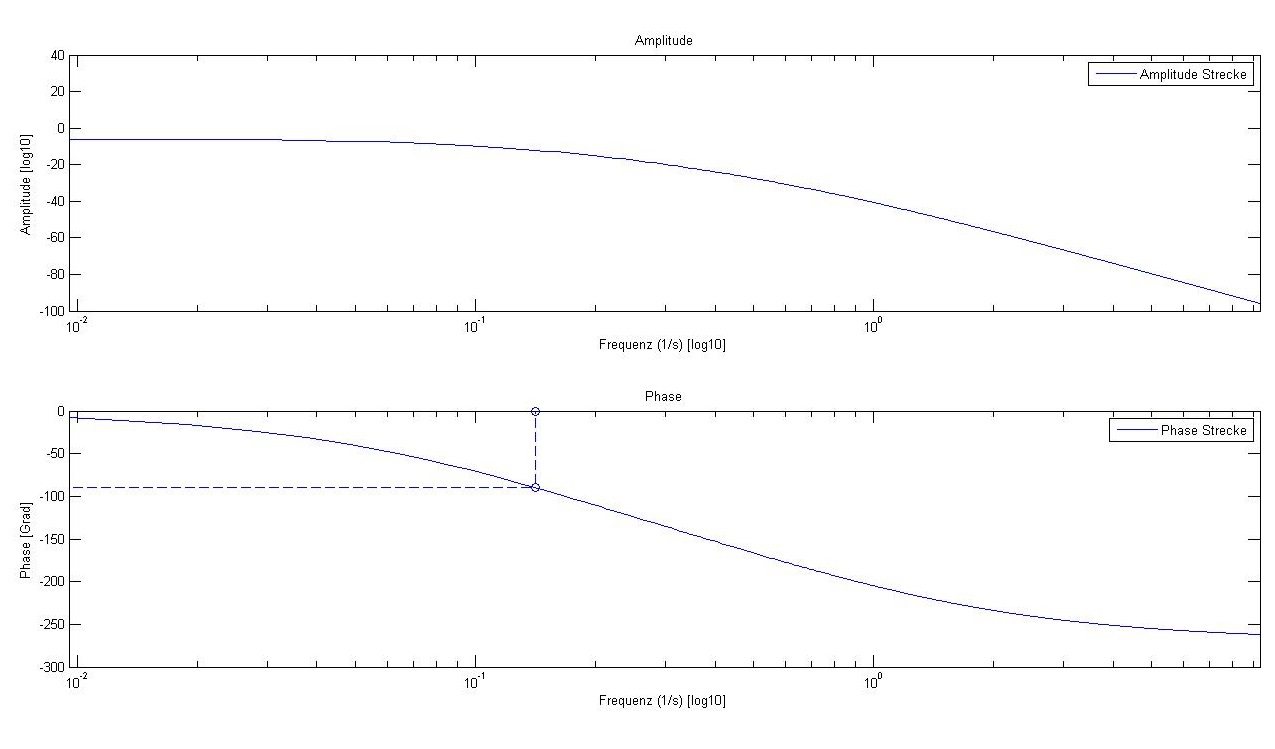
\includegraphics[width=1.0\textwidth]{PI_Step_01.jpg}
\caption{Amplituden- und Phasengang der Regelstrecke}	
\label{fig:PIStep1}	
\end{figure}

\newpage
Im n�chsten Schritt berechnet man mithilfe von $Tn$ und mit $Kr=1$ den offenen Regelkreis (rot dargestellt in Abbildung \ref{fig:PIStep2}).


\begin{figure}[h]	
\centering		
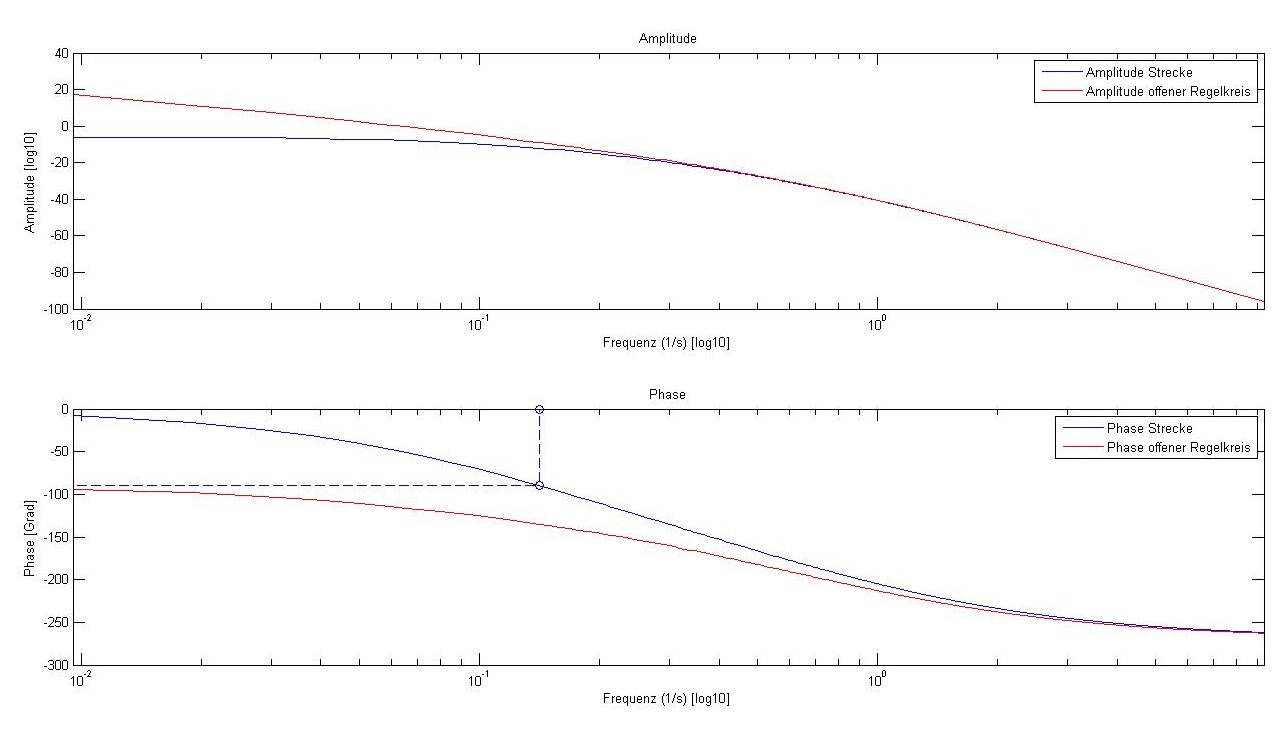
\includegraphics[width=1.0\textwidth]{PI_Step_02.jpg}
\caption{Frequenzgang der offenen Strecke}
\label{fig:PIStep2}
\end{figure}

Auf dem Phasengang des offenen Regelkreises (Abbildung \ref{fig:PIStep3}) wird nun die Frequenz bei $\phi_{Strecke}$ mithilfe der Tabelle \ref{table:Tab�berschwingen} auf Seite \pageref{table:Tab�berschwingen} gesucht (rot gestrichelte Linie). Die gefundene Frequenz ist $0.0611s^{-1}$.

\begin{figure}[h!]	
\centering		
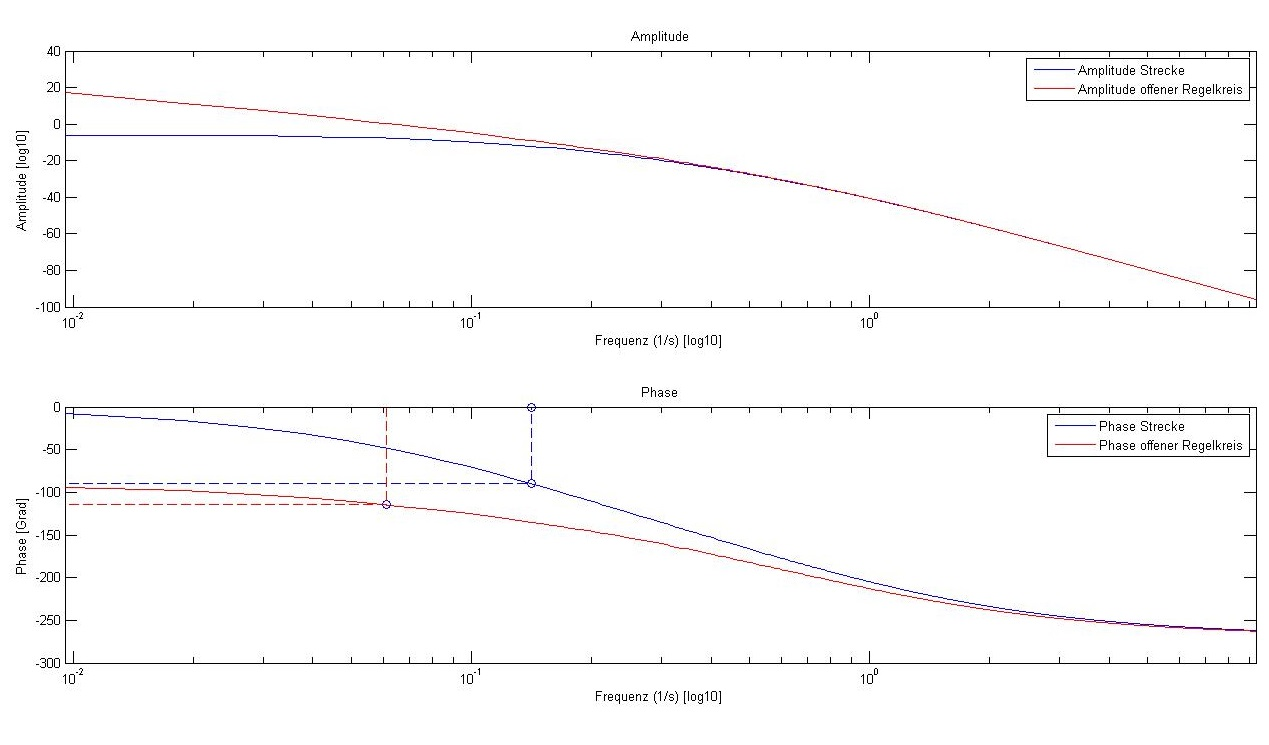
\includegraphics[width=1.0\textwidth]{PI_Step_03.jpg}
\caption{$\omega$ bei $\phi_{Strecke}$}	
\label{fig:PIStep3}	
\end{figure}

\newpage
Schliesslich wird die entsprechende Verst�rkung zur gefundenen Frequenz aus dem Amplitudengang des offenen Regelkreises herausgelesen (Abbildung \ref{fig:PIStep4}). In unserem Beispiel ergibt dies eine Verst�rkung von 1.0390.  Um diesen Faktor wird die Verst�rkung des Reglers gemindert, dies ergibt den letzten ben�tigten Parameter $Kr$.

\begin{figure}[h]	
\centering	
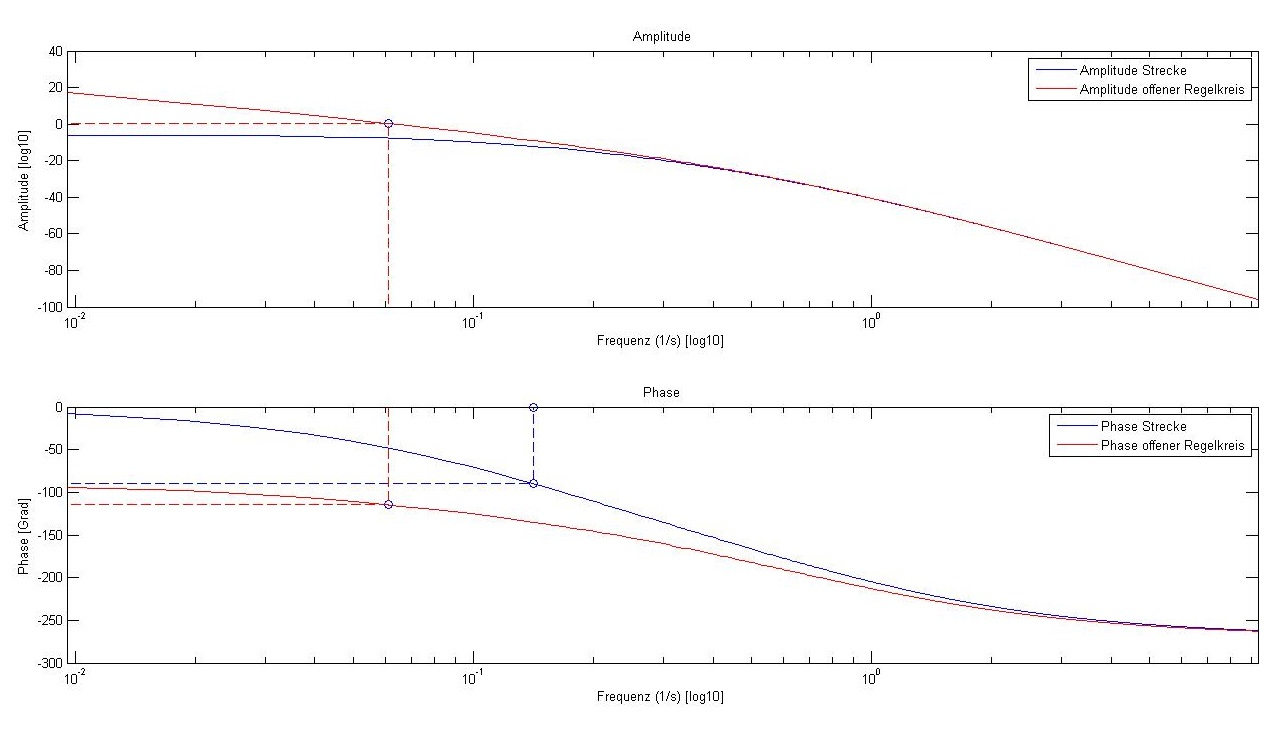
\includegraphics[width=1.0\textwidth]{PI_Step_04.jpg}
\caption{Bestimmung von $Kr$}	
\label{fig:PIStep4}	
\end{figure}

Die Endresultate dieser Berechnung sind:

$Tn = 7.0647s$\\
$Kr = 0.9625$

%\end{document}